%!TEX program = xelatex
%\documentclass[pra,twocolumn]{revtex4-1}
%\documentclass[preprint]{revtex4-1}
% \documentclass[a4paper]{article}
% \usepackate{cite}
\documentclass[11pt,a4paper]{article}
\usepackage{fontspec,amsmath,amssymb,bm}
\usepackage{xeCJK}
\usepackage{graphicx,float,subcaption}
\usepackage{url}
\usepackage[margin=2cm]{geometry}
\usepackage{listings}
\usepackage{lmodern}            % Use latin modern fonts
\usepackage{authblk}
\usepackage{SIunits}
\usepackage{braket}
%\usepackage{todonotes}
%\setmonofont{DejaVu Sans Mono}
\setCJKmainfont{cwTeX Q Ming}
% for chinese document
\renewcommand{\figurename}{圖}
\renewcommand{\tablename}{表格}

\title{Coherent population trapping by comb laser pulse}
\author{彭陸}
\affil[1]{國立台灣大學物理系}
\date{\today}
%\affiliation{National Taiwan University}

\begin{document}
\maketitle
\begin{abstract}
%TODO: find CPT paper G. Alzetta, A. Gozzini, M. Moi, and G. Orriols, Nuovo Ci- mento Soc. Ital. Fis., B 36,5 1976.
在這個研究中我們研究了銫原子的 $D_1$ 和 $d_2$ 光學吸收頻譜以及三、四以及五能階的簡化模型對超短脈沖鐳射所產生的 coherent population trappint (CPT) 現象。 利用 Liouville formalism (也可以稱為 Super operator formalism),我們開發出一個可以計算出 density matrix 隨時間的變化以及穩定時的狀態的演算法。利用這個演算法我們可以計算出 CPT 訊號的線寬、對比和 light shift,其結果可以和連續鐳射的情形比較。我們發現在超短脈沖的情況下,鐳射平均能量對線寬和 light shift 比連續鐳射的小很多。所以我們覺得超短脈沖 CPT 可以作為一個跟鐳射功率無關的頻率標準。此外,CPT 訊號的線寬正比於基態的弛緩速度(relaxation rate) $\Gamma$。\\
\end{abstract}

% \listoftodos
\section{簡介}
兩個基態能階與一個激發態能階用電場交聯在一起的現象稱微 coherent population trappint (CPT)。這種現象最早由Alzetta et al. \cite{Alzetta1976} 觀察到。CPT 現象可以運用於冷卻原子、magnetometry、 lasing without inversion 和原子頻率標準。在這篇報告中我們特別關心如何將CPT運用到頻率標準 \cite{Vanier2005}。CPT訊號可以用超短脈沖鐳射或連續鐳射激發。在這篇報告中我們會比較兩者的差異,並探討超短脈沖(光梳)CPT信號的應用。\\

在這篇報告中我們首先解釋CPT現象的原理。並解釋根據系統的能階圖如何將系統簡化成三、四或五能階模型。然後我們介紹在這篇報告中會研究的銫原子$D_1$、$D_2$系統。\\

在報告的第二部分鐘,我們會介紹一個我們用於計算 density matrix 的時間演化及穩態的微擾演算法。使用 Liouville formalism,我們可以計算出一個 super operator,這個 super operator 代表了一個微小時間間隔 $dt$ 裡光場對 density matrix 帶來的影響。Density matrix 的時間變化可以用這個 super operator 的冪次容易的計算出來。\\

在最後一段中,我們使用這個演算法計算簡化系統(三、四和五能階)以及包含所有 Zeeman 子能階的 $D_1$、$D_2$ 系統的CPT訊號。我們發現簡化系統的 CPT 訊號和完整 Zeeman 子能階的系統特性很相似。我們也比較超短脈沖光梳CPT和連續波CPT信號,發現光梳CPT信號鐳射平均功率對線寬和 light shift 的影響比連續波CPT信號的小很多。所以我們認為光梳CPT信號可以作為一個客觀的原子頻率標準。\\

% who have calculated ? Focus on what? Why we calculate this? how repetition rate effect CPT, clock standard. different focus. objective frequency. light shift, bandwidth.

\section{理論}
\subsection{Coherent Population Trapping (CPT)}
連續波的 Coherent popoulation trappint (CPT) 現象是使用兩個鐳射作用到一個 $\Lambda$ 系統上。 這個現象可以用鹼金屬原子容易的觀察到。在鹼金屬原子CPT中,鐳射光和兩個 $S_{1/2}$ 基態的超精細結構以及一個 $P$ 軌域的激發態作用,形成一個 $\Lambda$ 系統。如果兩道鐳射光的頻率和兩個基態和激發態之間共振,則會出現干涉的現象,原子就不會再吸收鐳射的能量,所以原子的能量吸。 如我把原子的能量吸收量對頻率作圖就會出現一個凹陷的圖形,這就是連續波CPT訊號。這個現象最早由 Alzetta et al. 在鈉原子使用 multi-mode dye laser\cite{Alzetta1976} 所觀察到。CPT現象的理論分析最早由 Orriols \cite{Orriols1979} 所提出。在這個報告中所研究的現象是由兩道鐳射和基態的 $F=3$ 、 $F=4$ 和 $P$ 能階的一個激發態作用。如果激發態選擇 $P_{1/2}$ , $F=3$ 和 $F=4$ 則稱為 $D_1$ 系統。如果激發態選擇 $P_{3/2}$ , $F=2$ 、 $F=3$ 、 $F=4$ 和 $F=5$ 則稱為 $D_2$ 系統。圖!!\\

在這篇文章中,右手方向(?)圓偏振的光會激發 $\Delta m_F = +1$。在有磁場時,因為 Zeeman 子能階的能量會分開所以必須考慮所有的 Zeeman 子能階,即使沒有磁場也得考慮 Zeeman 子能階因為他們也可能會影響系統的變化。從激發態因為 spontanious emission 或是碰撞(有加 buffer gas)衰變的電子可能會掉到所有的基態。取決於鐳射光的偏振,電子可能會被捕捉在$m_F = +4$ 或 $m_F = -4$ 的能階。在這種情況下,這些被捕捉的電子不再屬於 $\Lambda$ 系統,所以在嘗試簡化系統時必須要加入``陷阱能階''才能更準確地描述 CPT 現象\cite{Vanier1998}
。圖 \ref{fig:four_level} 顯示了簡化成四個能階的銫原子 $D_1$ 系統以及圓偏振($\sigma = +1$)的連續波雷射。電子囤積在能階 $F=4,m_F=4$ 因為它沒有被鐳射光連接到其他的 $P$ 能階。這些被捕捉的電子也會慢慢地重新分配到其他的 Zeeman 子能階上,因為基態能階之間有 relaxation rate $\gamma$。這種的能階表現得就像一個``leaky trap state''。圖\ref{fig:five_level}顯示了一個簡化成五能階的 $D_2$ 系統,除了 leaky trap state 以外在 $D_2$ 系統中還有個 $F=5,m_F=5$ 能階和 leaky trap state 被鐳射連接在一起,所以我們必須把它夾到簡化的系統中,所以形成了一個五能階的系統。\\

我們使用 density matrix 來分析。使用 Liouville-Von Neumann 方程式(式\ref{eq:lvn})可以描述 density matrix 的變化:\\

\begin{equation}
\label{eq:lvn}
\frac{\partial \rho}{\partial t} = \frac{i}{i\hbar} \left[ H,\rho \right]
\end{equation}
%\todo{Add Hamiltonian here}

\begin{figure}[H]
\centering
\begin{subfigure}[b]{0.3\textwidth}
\centering
\includegraphics[width=\textwidth]{small_system/three.pdf}
\caption{三能階系統}
\label{fig:three_level}
\end{subfigure}
\begin{subfigure}[b]{0.3\textwidth}
\centering
\includegraphics[width=\textwidth]{small_system/four.pdf}
\caption{四能階系統}
\label{fig:four_level}
\end{subfigure}
\begin{subfigure}[b]{0.3\textwidth}
\centering
\includegraphics[width=\textwidth]{small_system/five.pdf}
\caption{五能階系統}
\label{fig:five_level}
\end{subfigure}
\caption{四能階與五能階系統和銫原子$d_1$,$d_2$系統的比較}
\label{fig:analog}
\end{figure}

除了使用兩個連續波鐳射以外,我們也可以使用超短脈沖鐳射。因為超短脈沖鐳射的頻域範圍十分廣泛,所以即使在有磁場的情況下它也可以和所有的 Zeeman 子能階交互作用。這種情況下的 CPT 信號稱為光梳 CPT 信號。CW CPT 信號可以容易地用 rotating wave approximation 計算\cite{Vanier1998}\cite{Orriols1979}。Felinto et al 計算三能階的同調累積過程(? coherent accumulation process)\cite{Felinto2004}。在這篇報告中我們將計算擴充到銫原子的 $D_1$ 系統(32個 Zeeman 子能階) 以及 $D_2$ 系統(48個 Zeeman 子能階)並且將結果和連續波 CPT 信號比較。\\

\subsection{銫原子的 $D_1$ 和 $D_2$ 光學吸收譜線}

要能夠更準確地計算光梳 CPT 信號,必須考慮所有的 Zeeman 子能階,因為他們都會看超短脈沖鐳射寬廣的頻譜中的某些頻率作用。銫原子 D line 有兩個成分:$D_1$ line ($6^2s_{1/2}\Rightarrow 6^2P_{1/2}$ transition) 和 $D_2$ line ($6^2S_{1/2}\Rightarrow6^2P_{3/2}$ transition)。$D_2$ 系統在現今的原子光學研究中是比較重要的,因為它較常用於because it has a cycling transition that is used for cooling and trapping cesium.(?)\\

衰變速率(Decay rate) $\Gamma$ 代表了銫原子 D line 的自然線寬(FWHM),$D_1$ 和 $D_2$ 的 $\Gamma$ 分別是 $2\pi \cdot 4.575(12) \mega\hertz$ 和 $2\pi \cdot 5.234(13) \mega\hertz$。因為在實驗中有加入緩衝氣體,所以在模擬中 $D_1$ 和 $D_2$ 系統的衰變速率 $\Gamma$ 設定為 $700 \mega\hertz$ 以符合實驗情況。\\%\todo{reference}。\\

在 Hamiltonian 中的非對角項代表了銫原子和接近共振的鐳射光場的交互作用,其大小由 dipole 矩陣元素決定。$\Braket{F m_F | er | F^{\prime} m_F^{\prime}}$ 決定了兩個超精細能階的 dipole 矩陣元素 $\ket{ F m_F }$ and $\ket{ F^{\prime} m_F^{\prime}}$. 這些 dipole 矩陣元素可以用 Wigner-Eckart 定理來計算。\\

\begin{equation}
\Braket{ F m_F | er | F^{\prime} m_F^{\prime}} =\dots
\end{equation}

以下方程式是$F_g \Rightarrow F_e$ hyperfine 躍遷的 density matrix 的 master equation \cite{Steck2003}。

%\begin{widetext}
\begin{align}
\frac{\partial}{\partial t} \tilde{\rho}_{\alpha m_{\alpha},\beta m_{\beta}} = &
- \frac{i}{2} \left[ \delta_{\alpha e}\sum_{m_g} \Omega \left( m_{\alpha},m_g \right) \tilde{\rho}_{g m_g, \beta m_{\beta}} - \delta_{g \beta}\sum_{m_e} \Omega \left( m_{e},m_\beta \right) \tilde{\rho}_{\alpha m_\alpha, e m_{e}} \right.\nonumber\\ &+ \left. \delta_{\alpha g}\sum_{m_e} \Omega^{\star} \left( m_{e},m_\alpha \right) \tilde{\rho}_{e m_e, \beta m_{\beta}} - \delta_{e \beta}\sum_{m_g} \Omega^{\star} \left( m_{\beta},m_g \right) \tilde{\rho}_{\alpha m_\alpha, g m_{g}} \right] \label{eq:masterpumpfield}   \\
&-\delta_{\alpha e}\delta_{e \beta} \Gamma \tilde{\rho}_{\alpha m_{\alpha}, \beta m_{\beta}} \label{eq:masterdissipation1}\\
&- \delta_{\alpha e}\delta_{g \beta} \frac{\Gamma}{2} \tilde{\rho}_{\alpha m_{\alpha},\beta m_{\beta}}\label{eq:masterdissipation2}\\
&- \delta_{\alpha g}\delta_{e \beta} \frac{\Gamma}{2} \tilde{\rho}_{\alpha m_{\alpha}, \beta m_{\beta}} \label{eq:masterdissipation3}\\
&+ \delta_{\alpha g}\delta_{g \beta} \Gamma \sum_{q = -1}^{1} \left[ \tilde{\rho}_{e \left( m_{\alpha} + q \right), e \left(m_{\beta}+q  \right)} \braket{F_e \left( m_{\alpha}+q \right) | F_g 1 m_{\alpha} q} \braket{  F_e \left( m_{\beta} + q \right)  | F_g 1 m_{\beta} q }\right]\label{eq:masterdissipation4}\\
&+ i \left( \delta_{\alpha e} \delta_{g \beta} - \delta_{\alpha g}\delta_{e \beta} \right) \Delta\tilde{\rho}_{\alpha m_{\alpha}, \beta m_{\beta}} \label{eq:masterfreeevolution}\\
&- \gamma (\delta_{\alpha,S_{1/2}F=3}\delta_{\beta,S_{1/2}F=4}+\delta_{\alpha,S_{1/2}F=4}\delta_{\beta,S_{1/2}F=3}) \tilde{\rho}_{\alpha m_{\alpha}, \beta m_{\beta}}\label{eq:groundstaterelax}\\
&- \gamma \delta_{\alpha,S_{1/2}F=3}\delta_{\beta,S_{1/2}F=3} \sum_{m_{S_{1/2}F=4}} (\tilde{\rho}_{\alpha m_{\alpha}, \beta m_{\beta}} - \tilde{\rho}_{S_{1/2}F=4 m_{S_{1/2}F=4},S_{1/2}F=4 m_{S_{1/2}F=4} })\label{eq:groundstaterelax2}\\
&- \gamma \delta_{\alpha,S_{1/2}F=4}\delta_{\beta,S_{1/2}F=4} \sum_{m_{S_{1/2}F=3}} (\tilde{\rho}_{\alpha m_{\alpha}, \beta m_{\beta}} - \tilde{\rho}_{S_{1/2}F=3 m_{S_{1/2}F=3},S_{1/2}F=3 m_{S_{1/2}F=3} })\label{eq:groundstaterelax3}
\end{align}
%\end{widetext}

方程式 \ref{eq:masterpumpfield} 包含了和 pump field 有關的項,在這個方程式中 $\alpha$ 和 $\beta$ 代表超精細結構能階的量子數。$e$ 代表激發態($P$軌域能階),$g$ 代表激發態($S$軌域能階)。方程式 \ref{eq:masterdissipation1} 到方程式 \ref{eq:masterdissipation4} 是代表衰變的方程式。方程式 \ref{eq:masterfreeevolution} 是 Liouville-Von Neumann 運動方程式。方程式 \ref{eq:groundstaterelax} 到方程式 \ref{eq:groundstaterelax3} 是代表基態衰變的項。$\Omega$ 是拉比頻率。而 $\tilde{\rho}_{\alpha\beta} \equiv \rho_{\alpha\beta} \exp \left( -i \Delta_{\alpha\beta} t \right)$ 是 ``緩慢變動的coherence(slowly varying coherence)'',$\Delta_{\alpha\beta}$ 是能階 $\alpha$ 和能階 $\beta$ 之間的共振頻率。$\rho$ 是反對稱的, 表示 $\tilde{\rho}_{\alpha\beta} = \tilde{\rho}^{\ast}_{\alpha\beta}$. 一般而言, master equation 很難有解析解, 而在能階很多的情況下隨時間變化的 density matrix 是很耗費計算資源的。\\

%Equation \ref{eq:masterpumpfield} contain terms related to pump field, In this equation $\alpha$ and $\beta$ represent the hyperfine levels, $e$ means excited states ($P$ states), $g$ means ground states ($S$ states). The equations \ref{eq:masterdissipation1} to equation \ref{eq:masterdissipation4} are dissipation terms. Equation \ref{eq:masterfreeevolution} is the free evolution. Equations \ref{eq:groundstaterelax} to \ref{eq:groundstaterelax3} are terms related to ground state relaxation (PRINCIPLE OF GROUND STATE RELAX). $\Omega$ is the Rabi frequency between two magnetic sublevels. And $\tilde{\rho}_{\alpha\beta} \equiv \rho_{\alpha\beta} \exp \left( -i \Delta_{\alpha\beta} t \right)$ is a ``slowly varying coherence'', where $\Delta_{\alpha\beta}$ is the resonance frequency between state $\alpha$ and state $\beta$. $\rho$ is anti-symmetry, which means $\tilde{\rho}_{\alpha\beta} = \tilde{\rho}^{\ast}_{\alpha\beta}$. In general, the master equation is hard to treat analytically, a numerical solution of the time-dependent equation can be time-consuming if a large number of degenerate states are involved.\\

在接下來的討論中,我們介紹一種可以計算與超短脈沖作用的銫原子的 density matrix 隨時間變化以及穩定解的演算法。\\

\subsection{Liouvillian formalism}
為了要計算 density matrix 的時間變化,我們使用 Liouvillian formalism。利用接下來會介紹的演算法,我們可以計算出一個 super operator (或稱為 Liouville operator, tetradic matrix)。這個 super operator 代表了density matrix 在兩個脈沖之間的小時間間隔的變化。就像普通的 $n \times n$ 個元素的 operator 作用在 $n$ 維希爾伯特空間中的狀態向量一般,super operator 是對在 $n^2$ 維 Liouville 空間的 operator 或 density matrix 做數學變換。\\

例如,一個在 $n$-維希爾伯特空間 $\mathcal{H}_{n}$ 的 $n \times n$ operator $\hat{A}$,

\begin{equation}
\hat{\mathcal{A}} =
\begin{bmatrix}
\braket{ 1 | \hat{A}|1 } & \braket{ 1 | \hat{A}|2 } & \cdots & \braket{ 1 | \hat{A}|n } \\
\braket{ 2 | \hat{A}|1 } & \braket{ 2 | \hat{A}|2 } & \cdots & \braket{ 2 | \hat{A}|n } \\
\vdots  & \vdots  & \ddots & \vdots  \\
\braket{ n | \hat{A}|1 } & \braket{ n | \hat{A}|2 } & \cdots & \braket{ n | \hat{A}|n }
\end{bmatrix}
\end{equation}

$\hat{\mathcal{A}}$ 可以被表示成在 $n^2$ 維 Liouville 空間 $\mathcal{L}_{n^2}$ 裡的一個 $n^2$ 個元素的向量。\\

\begin{equation}
\hat{\mathcal{A}} =
\begin{bmatrix}
\braket{ 1 | \hat{A}|1 }\\
\braket{ 1 | \hat{A}|2 }\\
\braket{ 1 | \hat{A}|3 }\\
\vdots\\
\braket{ 1 | \hat{A}|n }\\
\braket{ 2 | \hat{A}|1 }\\
\vdots\\
\braket{ n | \hat{A}|n }\\
\end{bmatrix}
\end{equation}

使用這種把 operator 表示成在 $\mathcal{L}_{n^2}$ 的向量的方法。我們可以使用一個 $n^2 \times n^2$ 的矩陣 $\hat{\mathcal{S}}$ (共有 $n^4$ 個元素) 來變換這個向量。這個矩陣 $\hat{\mathcal{S}}$ 稱為一個 super operator (也可稱為 Liouville operator 或 tetradic matrix)。\\

\begin{equation}
\hat{\mathcal{S}} \left[ \hat{\mathcal{A}} \right] = \hat{\mathcal{B}}
\end{equation}

\begin{equation}
%\footnotesize
\begin{bmatrix}
\braket{ 1 | \hat{S}|1 } & \braket{ 1 | \hat{S}|2 } & \cdots & \braket{ 1 | \hat{S}|n^2 } \\
\braket{ 2 | \hat{S}|1 } & \braket{ 2 | \hat{S}|2 } & \cdots & \braket{ 2 | \hat{S}|n^2 } \\
\vdots  & \vdots  & \ddots & \vdots  \\
\braket{ n^2 | \hat{S}|1 } & \braket{ n^2 | \hat{S}|2 } & \cdots & \braket{ n^2 | \hat{S}|n^2 }
\end{bmatrix}
\begin{bmatrix}
\braket{ 1 | \hat{A}|1 }\\
\braket{ 1 | \hat{A}|2 }\\
\braket{ 1 | \hat{A}|3 }\\
\vdots\\
\braket{ 1 | \hat{A}|n }\\
\braket{ 2 | \hat{A}|1 }\\
\vdots\\
\braket{ n | \hat{A}|n }\\
\end{bmatrix}
=
\begin{bmatrix}
\braket{ 1 | \hat{B}|1 }\\
\braket{ 1 | \hat{B}|2 }\\
\braket{ 1 | \hat{B}|3 }\\
\vdots\\
\braket{ 1 | \hat{B}|n }\\
\braket{ 2 | \hat{B}|1 }\\
\vdots\\
\braket{ n | \hat{B}|n }\\
\end{bmatrix}
\end{equation}

\subsection{演算法}
在這篇報告中我們使用半古典的方式,將鐳射的電場表示為:

\begin{equation}
E(t) = E_{env}(t)\times  \frac{e^{-i\omega_c t}+e^{i\omega_c t}}{2}
\end{equation}
$E_{env}(t)$ 是電場 $E(t)$ 脈沖的包絡線而 $\omega_c$ 是載波頻率。\\

% explain condition of rotation wave approx and perturbation

我們所提出的演算法所用到的近似適用於以下條件:

\begin{enumerate}
  % \setlength{\itemsep}{1pt}
  % \setlength{\parskip}{0pt}
  % \setlength{\parsep}{0pt}
  \item 脈沖鐳射的頻寬比 S 軌域和 P 軌域的頻率差小很多。
%\item the bandwidth of pulse laser is much smaller than the frequency gap between the S orbital and P orbital.
\item $\int E(t) dt$,脈沖的面積夠小使得微擾可以收斂。
%\item $\int E(t) dt$, the area of the pulse is small enough so that the perturbation series can converge.
\end{enumerate}

Desntiy matrix 隨時間的變化是由 Liouville-Von Neumann 方程式來表示,我們可以用 super operator 的形式來表達他。把 desntiy matrix 的時間為分表達成 super operator $\mathcal{H}$ 作用到 density matrix上。\\

\begin{equation}
i \hbar \frac{\partial}{\partial t}\rho = \mathcal{H}[\rho] \equiv [H,\rho] \equiv H\rho - \rho H
\end{equation}

使用 Liouville formalism 讓我們可以根據 master equation eq.\ref{eq:masterpumpfield} 把 decoherent 的項事後加入到 super operator 中。\\

定義 ``slowly varying coherence'' $\tilde{\rho}_{\alpha\beta} \equiv \rho_{\alpha\beta} \exp \left( -i \omega_{\alpha\beta} t \right)$。如果量子態 $\alpha$ 和 $\beta$ 不一樣,則 $\omega_{\alpha\beta}$是載波頻率。如果量子態 $\alpha$ 和 $\beta$ 一樣,則 $\omega_{\alpha\beta} = 0$。當脈沖鐳射的載波頻率被 slowly varying coherence 的 exponential 相抵消掉後,再使用 rotating wave approximation 消去高頻的項。這個super operator可以分成兩個部分,第一個部分 $\mathcal{A}$ 則和電場無關, 另一個部分 $\mathcal{B} E_{env} \left( t \right)$ 正比於電場 $E \left( t \right)$。\\

\begin{equation}
\frac{d\tilde{\rho}}{dt} = \left( \mathcal{A} + E_{env}\left( t \right) \mathcal{B}\right) \left[  \tilde{\rho}\right]
\end{equation}

以三個能階的 $\Lambda$ 系統為例,$\left| 2 \right\rangle,\left| 3 \right\rangle$ 是兩個比較低的能階,$\left| 1 \right\rangle$ 是比較高的能階。 這個系統的 Hamiltonian 是:\\

\begin{align}
H &= H_0+H_{int}\nonumber \\
&=
\left(
\begin{array}{ccc}
\hbar \omega_1 & 0&0\\
0& \hbar \omega_{2}&0\\
0&0&0
\end{array}
\right)\nonumber\\  &+
\left(
\begin{array}{ccc}
0& \mu_{12} E(t)&\mu_{13}E(t)\\
\mu_{12}E(t) &0&0\\
\mu_{13}E(t)&0&0
\end{array}
\right)
\end{align}

% With the Von Neumann equation for time evolution $i \hbar \frac{\partial \rho}{\partial t} = [H,\rho]$.
$\mu_{ij}$ 是 $i\Rightarrow j$ 躍遷的 dipole moment。這個 density matrix 的運動方程式是:\\
\begin{align}
\label{eq:timeevo3}
i \hbar \dot{\rho_{11}} &= -\mu_{12}E(t)\rho_{21}-\mu_{13}E(t)\rho_{31}+\mu_{12}E(t)\rho_{12}+\mu_{13}E(t)\rho_{13}\nonumber\\
i \hbar \dot{\rho_{22}} &= -\mu_{12}E(t)\rho_{12}+\mu_{12}E(t)\rho_{21}\nonumber\\
i \hbar \dot{\rho_{33}} &= -\mu_{13}E(t)\rho_{13}+\mu_{13}E(t)\rho_{31}\nonumber\\
i \hbar \dot{\rho_{12}} &= \hbar\omega_{2}\rho_{12}-\mu_{12}E(t)\rho_{22}-\mu_{13}E(t)\rho_{32}+\mu_{12}E(t)\rho_{11}-\rho_{12}\hbar\omega_{1}\nonumber\\
i \hbar \dot{\rho_{13}} &= \hbar\omega_1\rho_{13}-\mu_{12}E(t)\rho_{23}-\mu_{13}E(t)\rho_{33}+\mu_{13}E(t)\rho_{11}\nonumber\\
i \hbar \dot{\rho_{23}} &= -\mu_{12}E(t)\rho_{13}-\hbar\omega_{2}\rho_{23}+\mu_{13}E(t)\rho_{21}\nonumber\\
\end{align}

定義 slowly varying coherence $\tilde{\rho}_{\alpha\beta}$,以使用 rotating wave approximation (RWA):\\
\begin{align*}
\rho_{12} &= \tilde{\rho}_{12}e^{i\omega_c t}\\
\rho_{13} &= \tilde{\rho}_{13}e^{i\omega_c t}\\
\rho_{23} &= \tilde{\rho}_{23}
\end{align*}
$\omega_c$是脈沖鐳射的載波頻率。把這些項帶入運動方程式,並使用 rotating wave approximation 以移除高頻項。使用之前提到定義 slowly varying coherence 的方法,rotating wave approximation 也可以用到有 Zeeman 子能階的情況。\\

再做完 rotating wave approximation 之後,加入衰變項以及基態的方鬆(relaxation),方程式\ref{eq:timeevo3} 變成:\\
%After the rotating wave approximation is applied and dissipation terms and the ground state relaxation terms added, eq.\ref{eq:timeevo3} becomes:

\begin{align}
\label{eq:timeevo3}
\dot{\rho}_{11} &= -2\Gamma \rho_{11} + \Omega_{12}(t)\Im \left[ \tilde{\rho}_{12} \right]+\Omega_{13}(t)\Im \left[ \tilde{\rho}_{13} \right]\nonumber\\
\dot{\rho}_{22} &= \Gamma \rho_{11} -\Omega_{12}(t)\Im \left[ \tilde{\rho}_{12} \right] - \gamma \left( \rho_{22} - \rho_{33} \right)\nonumber\\
\dot{\rho}_{33} &= \Gamma \rho_{11} -\Omega_{13}(t)\Im \left[ \tilde{\rho}_{13} \right] - \gamma \left( \rho_{33} - \rho_{22} \right)\nonumber\\
\dot{\tilde{\rho}}_{12} &= -\frac{1}{2}\Gamma\tilde{\rho}_{12} +i \frac{\Omega_{12}(t)}{2}\left( \rho_{22} - \rho_{11} \right) + i \tilde{\rho}_{12} \left( \omega_1 - \omega_2 -\omega_c \right) \nonumber\\
\dot{\tilde{\rho}}_{13} &= -\frac{1}{2}\Gamma\tilde{\rho}_{13} +i \frac{\Omega_{13}(t)}{2} \left( \rho_{33} - \rho_{11} \right) + i \tilde{\rho}_{13} \left( \omega_1 - \omega_3 -\omega_c \right)\nonumber\\
\dot{\tilde{\rho}}_{23} &= -\gamma\tilde{\rho}_{23} + i \frac{\Omega_{12}(t)}{2}\tilde{\rho}_{13} -i \frac{\Omega_{13}(t)}{2}\tilde{\rho}_{21}+i\omega_2 \tilde{\rho}_{23}\nonumber\\
\end{align}

$\Omega_{ij}(t) = \frac{\mu_{ij}E_{env}(t)}{\hbar}$ 是拉比頻率。\\

如果我們把 density matrix 展開成一個向量,例如讓第 $(i,j)$ 個 density matrix 矩陣元素變成第 $(i-1)n+j$ 個向量元素。$n$ 是希爾伯特空間的維度。\\

\begin{equation}
\tilde{\rho} =
\begin{bmatrix}
\rho_{11}&
\tilde{\rho}_{12}&
\tilde{\rho}_{13}&
\hdots&
\tilde{\rho}_{21}&
\rho_{22}&
\hdots&
\rho_{33}
\end{bmatrix}^{T}
\end{equation}

可以把 density matrix 變成 density matrix 的時間微分的 super operator 可以表示成:\\

\begin{equation}
\dot{\rho}(t) =  \mathcal{S}(t) \left[ \rho(t) \right]
\end{equation}
%\begin{widetext}
%  \footnotesize
\begin{equation}
\label{eq:ASO}
\mathcal{S}(t) =
\begin{bmatrix}
-2\Gamma & \frac{\Omega_{12}(t)}{2i} &\frac{\Omega_{13}(t)}{2i} & -\frac{\Omega_{12}(t)}{2i} & 0&0&-\frac{\Omega_{13}(t)}{2i}&0&0 \\
-i \frac{\Omega_{12}(t)}{2} &i\Delta\omega_1-\frac{\Gamma}{2}&0&0&i \frac{\Omega_{12}(t)}{2}&0&0&0&0\\
-i \frac{\Omega_{13}(t)}{2} &0&i\Delta\omega_2-\frac{\Gamma}{2}&0&0&0&0&0&i \frac{\Omega_{13}(t)}{2}\\
i \frac{\Omega_{12}(t)}{2} &0&0&-i\Delta\omega_1-\frac{\Gamma}{2}&-i \frac{\Omega_{12}(t)}{2}&0&0&0&0\\
\Gamma&- \frac{\Omega_{12}(t)}{2i}&0&\frac{\Omega_{12}(t)}{2i}&-\gamma&0&0&0&\gamma\\
0&0&i \frac{\Omega_{12}(t)}{2}&-i \frac{\Omega_{13}(t)}{2}&0&-\gamma+i\omega_{2}&0&0&0\\
i \frac{\Omega_{13}(t)}{2} &0&0&0&0&0&-i\Delta\omega_2-\frac{\Gamma}{2}&0&-i \frac{\Omega_{13}(t)}{2}\\
0&i \frac{\Omega_{13}(t)}{2}&0&0&0&0&-i \frac{\Omega_{12}(t)}{2}&-\gamma-i\omega_{2}&0\\
\Gamma&0&- \frac{\Omega_{13}(t)}{2i}&0&\gamma&0&\frac{\Omega_{13}(t)}{2i}&0&-\gamma\\
\end{bmatrix}
\end{equation}
%\end{widetext}

在 super operator eq.\ref{eq:ASO} 中,$\Delta\omega_1 = \omega_1-\omega_2-\omega_{c}$ 而且 $\Delta\omega_2 = \omega_1-\omega_3-\omega_{c}$。因為 density matrix 是反對稱的,所以 super operator 有個特性是 $\mathcal{S}_{(i-1)n+j,(k-1)n+l} = \mathcal{S}^{*}_{(j-1)n+i,(l-1)n+k}$。Super operator $\mathcal{S}$ 可以分成兩部分:$\mathcal{A}$ 是和時間無關的,包含了衰變項、基態弛緩(relaxation)和 free evolution。$\mathcal{B}E_{env}(t)$則包含了pump field 相關的項(有$E_{env}(t)$ 或 $\Omega_{ij}(t)$)。其他系統的 super operator $\mathcal{S}$ 可以用一樣方法建構出來。\\

\begin{figure}[H]
\centering
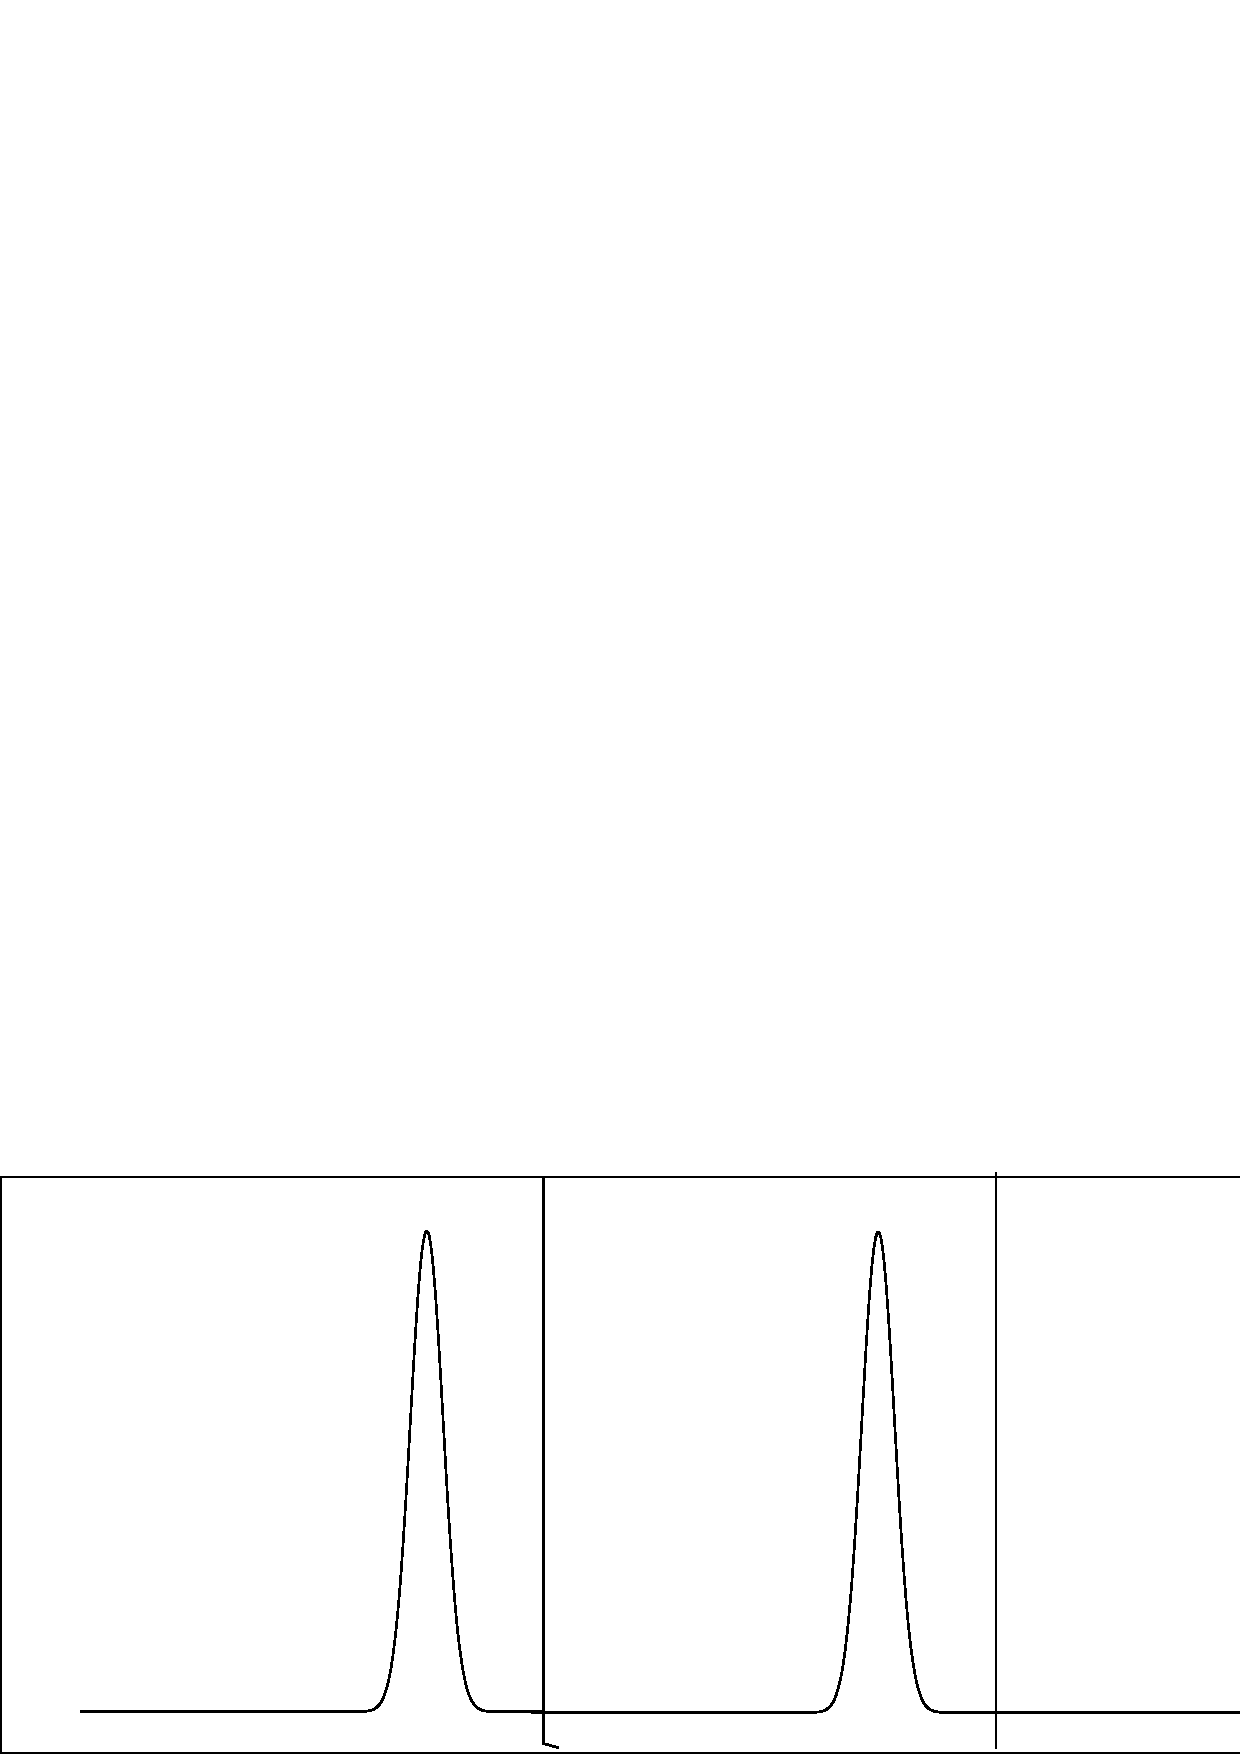
\includegraphics[width=7cm]{pulses.pdf}
\caption{Pulses}
\label{fig:pulses}
\end{figure}
\begin{figure}[H]
\centering
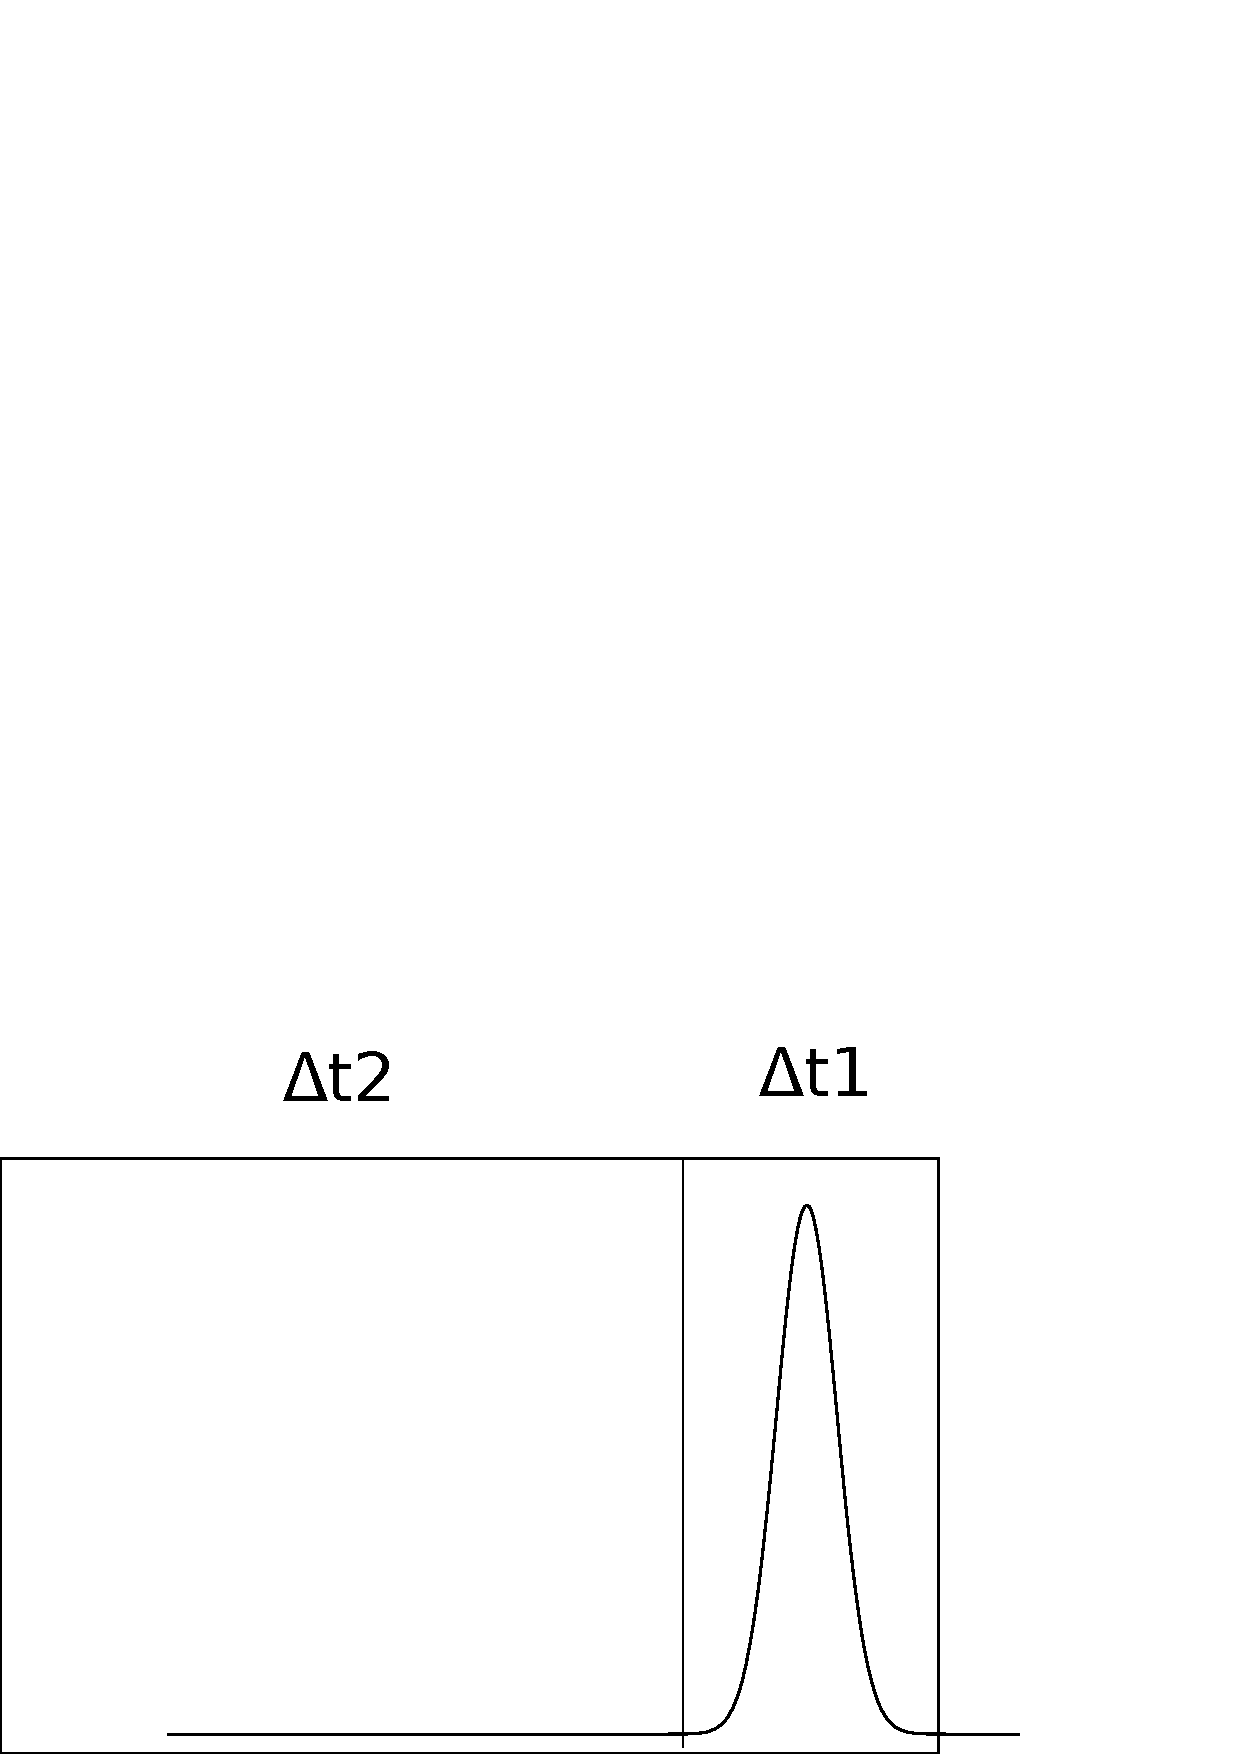
\includegraphics[width=6cm]{pulse.pdf}
\caption{Pulse}
\label{fig:pulse}
\end{figure}

脈沖鐳射在時間領域上可以分成很多小段,如圖\ref{fig:pulses}所示。每個時間小段又可以進一步分成兩部分:一部分長 $\Delta t_1$ 的段落包含了鐳射脈沖;另一段長度 $\Delta t_2$ 的段落的電場小到可以忽略。如圖\ref{fig:pulse}所示。\\

如果 density matrix 在脈沖開始之前($t=0$)是 $\tilde{\rho}(0)$。定一兩個 super operator:\\

\[
\tilde{\rho}(\Delta t_1) = \mathcal{P}^{\prime} \left[ \tilde{\rho}(0) \right]
\]
\[
\tilde{\rho}(\Delta t_1+\Delta t_2) = \mathcal{P} \left[\tilde{\rho}(\Delta t_{1})\right] = \mathcal{P} \mathcal{P}^{\prime} \left[\tilde{\rho}(0)\right]
\]

因為在 $\Delta t_1<t<\Delta t_1+\Delta t_2$ 時可以當作沒有電場,所以這時候的運動方程式是 $\dot{\tilde{\rho}} = \mathcal{A} \left[\tilde{\rho}\right]$。所以 $\tilde{\rho}(\Delta t_1+\Delta t_2) = e^{i \mathcal{A} \Delta t_{2}} \left[ \tilde{\rho}(\Delta t_{1}) \right] $, 在這裡 super operator 的指數算法和一般的矩陣指數一樣。\\

\[
\mathcal{P} = e^{i \mathcal{A} \Delta t_2}
\]

有電場的部分 $\mathcal{P}^{\prime}$ 可以使用微擾法來解。定義 $\tilde{\rho}_n (t)$ 為運動方程式 $\dot{\tilde{\rho}} = \left( A + B E_{env}(t) \right) \left[ \tilde{\rho} \right] $ 在時間範圍 $0< t < \Delta t_{1}$ 內第 $n$ 階的解。定義另一個 super operator $F(t)_{n} \tilde{\rho}(0) = \tilde{\rho}_{n}(t)$, 這個 super operator 可以把 desity matrix 的初始狀態 $\tilde{\rho}(0)$ 轉變成第 $n$ 階的解 $\tilde{\rho}_n (t)$。\\

如果 density matrix 的初始狀態 $\tilde{\rho}(0)$ 已經知道。第0階解答設成 $\tilde{\rho}_{0} (t) = e^{i A t} \tilde{\rho}(0)$。下一階的解答可以可以用微擾法獲得:\\

\begin{equation}
\label{eq:perturb}
\tilde{\rho}_{n+1}(t) = \int_0^{t} \left( \mathcal{A}+\mathcal{B} E_{env}(\tau) \right) \tilde{\rho}_n(\tau)\:d\tau, 0<t<\Delta t_1
\end{equation}

把 $\tilde{\rho}_n(t)$ 替換成 $F_n(t)\tilde{\rho}(0)$,方程式\ref{eq:perturb} 變成:\\

\begin{equation}
F_{n+1}(t)\tilde{\rho}(0) = \int_0^{t} \left( \mathcal{A}+\mathcal{B} E_{env}(\tau) \right) F_n(\tau)\tilde{\rho}(0)\:d\tau, 0<t<\Delta t_1
\end{equation}

把兩邊的常數矩陣 $\tilde{\rho}(0)$ 同除掉。\\

\begin{equation}
\label{eq:f}
F_{n+1}(\Delta t_1) = \int_0^{\Delta t_1} \left( \mathcal{A}+\mathcal{B} E_{env}(t) \right) F_n(t)\:dt
\end{equation}

$F_0(t) = e^{-iAt}$ 和 $F_{n}(0)$ 是單位矩陣 $I$, 方程式\ref{eq:f} 和初始條件 $\tilde{\rho}(0)$無關。所以$\mathcal{P}^\prime = \lim_{n\rightarrow \infty}F_{n}(\Delta t_{1})$。\\

Desnity matrix 的演化可以使用 $\mathcal{P}\mathcal{P}^\prime \left[ \tilde{\rho} \right]$ 計算。經過 $n$ 個脈沖的 density matrix 變成 $\left(\mathcal{P} \mathcal{P}^{\prime} \right)^{n} \left[ \tilde{\rho} \right]$。density matrix 的穩定解可以用 $\left(\mathcal{P} \mathcal{P}^{\prime} \right)\left[ \tilde{\rho}_{\mbox{steady state}} \right] = \tilde{\rho}_{\mbox{steady state}}$ 計算。\\

\section{數值計算結果}
根據上述的演算法,我們寫了一個程式。這個程式使用了 Enthought Python Distribution (EDP) 因為這個 python 版本的矩陣運算使用了 Intel math kernel 函式庫 (MKL) 以提供多核心的矩陣運算。另外在效能瓶頸的部分我們使用 C 語言來增進效能。這個程式運行在一個每個節點有24GB記憶體的 cluster 上。在我們的程式裡,所有有關銫原子的數值都來自 Ref.\cite{Steck2003}。\\

所有 P 和 S 軌域的 Zeeman 子能階都有被考慮。$D_1$ 譜線有 32 個能階;$D_2$ 譜線則有 48 個能階。在 48 個子能階的情況下, density matrix 就有 2304 個元素,而 super operator就會有 5308416 個元素。而在每一個時間間隔裡都必須使用不一樣的 super operator,所以這個演算法需要夠大的記憶空間。\\

在 $D_1$ 譜線的情況下,脈沖鐳射的載波頻率被調整到 $6^2S_1/2, F=3$ 和 $6^2P_{1/2}$ 的頻率差;在 $D_2$ 譜線的情況下載波頻率則是 $6^2S_1/2 , F=3$ 和 $6^2P_{3/2} , F=3$ 的頻率差。Repetition rate 是 $0.919263177 \giga\hertz$ ,這是 $6^2S_1/2$ $F=3$ 和 $6^2S_1/2$ $F=4$ 頻率差的 $\frac{1}{10}$。\\

為了符合實驗的情況,衰變頻率 $\Gamma$ 則是 $7 \times 10^8 \hertz$。鐳射脈沖的時間寬度 FWHM 則是 $-27.7\femto\second$,脈沖的包絡線是高斯函數 $C e^{ - \frac{t^2}{2 \sigma^{2}} }$, $\sigma = 20 \times 10^{-15} \second$。\\

% $\gamma	= 5\hertz$ and $\gamma = 1000\hertz$ is calculated.\\
%why select these parameters

\subsection{三、四和五能階模型}

我們先使用之前所描述的演算法來計算這些簡化模型的光梳 CPT 信號。三能階和四能接系統的差異在於因為三能階系統沒有 trap state,所以即使不考慮基態弛緩也會有 CPT 信號。然而,在四能階獲五能階系統中,如果不考慮基態弛緩的話,不管 repetition rate 如何,在 ensemble 中所有原子的電子都被困在 trap state 中。沒有原子的電子會處在高能量的能階,如圖\ref{fig:four_level_result_nogamma}所示。在 $D_2$ 系統的簡化五能階系統中,所有原子的電子都被困在 trap state 和 $F=5, m_f=5$ 中,所以高能量的能階居量變成一個獨立於 repetition rate 的常數,如圖\ref{fig:five_level_result_nogamma}所示。\\

 %explain how laser frequency is shifted
 \begin{figure}[H]
 \centering
 \begin{subfigure}[b]{0.45\textwidth}
 \centering
 \includegraphics[width=\textwidth]{small_system/four_level_1000_no_gamma.pdf}
 \caption{$\gamma = 0$ 的四能階系統}
 \label{fig:four_level_result_nogamma}
 \end{subfigure}
 \begin{subfigure}[b]{0.45\textwidth}
 \centering
 \includegraphics[width=\textwidth]{small_system/five_level_10_nogamma.pdf}
 \caption{$\gamma = 0$ 的五能階系統 }
 \label{fig:five_level_result_nogamma}
 \end{subfigure}
 \caption{四能階與五能階系統的光梳 CPT 信號:$\gamma = 0$ 的四能階和五能階 $P$ 軌域(高能量的能階)居量對時間和 repetition rate 作圖,只對高能量的能階作圖是因為實驗所觀察到的螢光是正比於高能量能階的居量。系統一開始是處於全部低能階的狀態,在四能階的系統中,高能階的居量漸漸的跑到位於低能階的 trap state,所以最後趨近於0。而五能階系統的所有居量最後跑到位於低能階 trap state 和 $F=5, m_f=5$ 中,所以高能階的居量最後變成常數。}
 \label{fig:nogamma}
 \end{figure}

 \begin{figure}[H]
 \centering
 \begin{subfigure}[b]{0.3\textwidth}
 \centering
 \includegraphics[width=\textwidth]{small_system/three_level_1000.pdf}
 \caption{三能階系統}
 \label{fig:three_level_result}
 \end{subfigure}
 \begin{subfigure}[b]{0.3\textwidth}
 \centering
 \includegraphics[width=\textwidth]{small_system/four_level_1000.pdf}
 \caption{四能階系統}
 \label{fig:four_level_result}
 \end{subfigure}
 \begin{subfigure}[b]{0.3\textwidth}
 \centering
 \includegraphics[width=\textwidth]{small_system/five_level_1000.pdf}
 \caption{五能階系統}
 \label{fig:five_level_result}
 \end{subfigure}
 \caption{數值結果:$P$ 軌域居量對 repetition rate 以及時間做圖,顯示了 CPT 信號對時間的變化。}
 \label{fig:small_system_result}
 \end{figure}

 \subsection{基態弛緩 $\gamma$ 的影響}
$D_2$ 譜線的光梳 CPT 信號的線寬和對比的數值結果呈現在圖\ref{fig:gamma_relation}中。如圖\ref{fig:gamma_relation}所示,線寬和基態弛緩的系數$\gamma$呈正比。而當$\gamma$上升時,對比則單調下降。

\begin{figure}[H]
\centering
\begin{subfigure}[b]{0.6\textwidth}
\centering
\includegraphics[width=\textwidth]{d2_gamma/linewidth.eps}
\caption{linewidth vs $\gamma$}
\label{fig:linewidth_gamma}
\end{subfigure}\\
\begin{subfigure}[b]{0.6\textwidth}
\centering
\includegraphics[width=\textwidth]{d2_gamma/contrast.eps}
\caption{contrast vs $\gamma$}
\label{fig:contrast_gamma}
\end{subfigure}
\caption{d2 line linewidth and contrast vs $\gamma$}
\label{fig:gamma_relation}
\end{figure}

\subsection{連續波鐳射和光梳鐳射CPT信號的比較}
我們計算了$D_1$和$D_2$譜線的光梳鐳射(一道鐳射)和連續波鐳射(兩道CW鐳射)的線寬、對比和light shift,並且比較相同平均能量的連續波鐳射和光梳鐳射的資料。基態弛緩系數$\gamma$設定為$5 \hertz$以符合實驗情況。在計算中,我們調變脈沖鐳射的 repetition rate;對於連續波鐳射我們則同時改變兩道連續波鐳射的頻率(一道鐳射增加$\Delta f$的頻率時,另一道就減少$\Delta f$)以模擬 AMO 調變的情形。\\

\begin{figure}
\centering
\begin{subfigure}[b]{0.6\textwidth}
\centering
\includegraphics[width=\textwidth]{d1_cw_p/linewidth.eps}
\caption{$D_1$連續波和脈沖鐳射線寬比較}
\label{fig:d1linewidth}
\end{subfigure}\\
\begin{subfigure}[b]{0.6\textwidth}
\centering
\includegraphics[width=\textwidth]{d1_cw_p/contrast.eps}
\caption{$D_1$連續波和脈沖鐳射對比比較}
\label{fig:d1contrast}
\end{subfigure}\\
\begin{subfigure}[b]{0.6\textwidth}
\centering
\includegraphics[width=\textwidth]{d1_cw_p/lightshift.eps}
\caption{$D_1$連續波和脈沖鐳射 light shift 比較}
\label{fig:d1lightshift}
\end{subfigure}
\caption{$D_1$ 連續波和脈沖鐳射CPT信號比較}
\label{fig:cwpd1}
\end{figure}

\begin{figure}
\centering
\begin{subfigure}[b]{0.6\textwidth}
\centering
\includegraphics[width=\textwidth]{d2_cw_p/linewidth.eps}
\caption{$D_2$連續波和脈沖鐳射線寬比較}
\label{fig:d2linewidth}
\end{subfigure}\\
\begin{subfigure}[b]{0.6\textwidth}
\centering
\includegraphics[width=\textwidth]{d2_cw_p/contrast.eps}
\caption{$D_2$連續波和脈沖鐳射對比比較}
\label{fig:d2contrast}
\end{subfigure}\\
\begin{subfigure}[b]{0.6\textwidth}
\centering
\includegraphics[width=\textwidth]{d2_cw_p/lightshift.eps}
\caption{$D_2$連續波和脈沖鐳射 light shift 比較}
\label{fig:d2lightshift}
\end{subfigure}
\caption{$D_2$連續波和脈沖鐳射 CPT 信號比較}
\label{fig:cwpd2}
\end{figure}

在圖 \ref{fig:cwpd1}和圖 \ref{fig:cwpd2}中,我們比較了 $D_1$ 和 $D_2$ 譜線的 CPT 信號。對於 $D_1$ 和 $D_2$ 譜線兩者而言,光梳 CPT 信號的線寬都比較窄,如圖 \ref{fig:d1linewidth} 和圖 \ref{fig:d2linewidth} 所示。光梳 CPT 信號的線寬都小於 $3 \hertz$ 而連續波鐳射的 CPT 線寬則大得多。至於對比,$D_1$ 譜線的 CPT 信號對比隨著平均能量增加而增加,連續波鐳射與脈沖鐳射都是如此。然而對於 $D_2$ 譜線而言。CW CPT的對比在一定能量之後就變得很小,如圖 \ref{fig:d2contrast}所示,這是因為比較高的鐳射能量使得 trap state ($F=5, m=5$ for $\sigma = +1$)增加($10^{-6}$),並且在其弛緩時產生 decoherence。Vanier et al. 也在文獻中描述過這個現象\cite{Vanier1998}。脈沖鐳射的情況下 trap state 的居量小的多($1 \times 10^{-10}$數量級)。脈沖 CPT 的 light shift 也比連續波鐳射的 CPT light shift 要小得多,如圖 \ref{fig:d1lightshift} 和圖 \ref{fig:d2lightshift} 所示。

% The simulation results of CW and pulse laser CPT signal are compared. The results are in figure \ref{fig:cwpd1} and \ref{fig:cwpd2}. For both $D_1$ and $D_2$ CPT line width are smaller for comb CPT signal, as shown in figure \ref{fig:d1linewidth} and \ref{fig:d2linewidth}. Line width of comb CPT signal is under $3 \hertz$ in simulated laser power range, while CW CPT line width is much larger. As for contrast, for $D_1$ CPT, contrast increase as laser power increase for both CW and comb CPT signal, see figure \ref{fig:d1contrast}. However for $D_2$ case, contrast of CW CPT signal drop after certain laser power, as shown in figure \ref{fig:d2contrast}, that is because higher laser power causes the population of trap state ($F=5, m=5$ for $\sigma = 1$) to rise ($10^{-6}$), which create decoherence while it relax. This phenomenon is also found by Vanier et al. \cite{Vanier1998}. The population of trap state in pulse laser case is much smaller (of order $1 \times 10^{-10}$). Pulse CPT signal also has a much smaller light shift compare to CW CPT, as shown in figure \ref{fig:d1lightshift} and figure \ref{fig:d2lightshift}.\todo{explain jitter}

\section{結論}
總結而言,我們開發了一個計算包含所有 Zeeman 子能階的光梳 CPT 信號的演算法。光梳 CPT 的線寬以及 light shift 都比連續波鐳射 CPT 的要小很多。簡化的四能階以及五能階系統保留了考慮所有 Zeeman 子能階的系統的一些定性的特性。
% In conclusion we present an effective algorithm to calculate comb CPT signal taking account of all Zeeman sublevels. The line width and light shift of comb CPT signal is much smaller its counterpart CW CPT signal. Some features present in full Zeeman sublevels simulation do not appear in four or five level model\todo{verify}.
\bibliography{reference}{}
\bibliographystyle{plain}
\end{document}
